\chapter{Analýza}

Po preskúmaní možností pre vykonanie podrobnej analýzy nasadenia NEL som podľa vypracovaného návrhu implementoval potrebné nástroje.
Úlohou týchto nástrojov je dopracovať sa k stanoveným cieľom mojej práce.  
Najskôr v tejto kapitole popisujem svoju prácu z hľadiska toho, čo bolo implementované.
Potom v sekcií \ref{sec:results} prezentujem jej celkové výsledky.


\section{Implementácia nástrojov pre analýzu}

Potrebné nástroje podľa návrhu práce (viď kapitolu \ref{possible-analysis-strategies}) predstavujú implementované skripty pre dve rozdielne metódy analýzy:
\begin{enumerate}
    \item Práca s HTTP Archive:
    \begin{itemize}
        \item[(a)] získať \textit{historické} dáta, 
        \item analyzovať ich a vyprodukovať výsledné metriky,
        \item výsledky podľa potreby vhodne vizualizovať.
    \end{itemize}

    \item Automatizované prehliadanie súčasného webu:
    \begin{itemize}
        \item[(b)] získať \textit{súčasné} dáta,
        \item analyzovať ich a vyprodukovať výsledné metriky, 
        \item výsledky podľa potreby vhodne vizualizovať.
    \end{itemize}
\end{enumerate}

Skutočnosť, že sa tieto dve metódy odlišujú iba v spôsobe získavania vstupných dát som využil pri návrhu skriptov.
Na začiatok som teda definoval štruktúru výstupných dát z prvého kroku oboch metód.
Spoločná štruktúra dát umožňuje implementovať zvyšné dva kroky pre obe metódy rovnako.
Tabuľka \ref{tab:analysis-data-structure} v prílohách túto štruktúru popisuje. 
% Bližšie ju popisuje nasledujúca sekcia o implementácií nástroja pre HTTP Archive.

\subsection{Skript pre prácu s HTTP Archive}

Vzhľadom na to, že som sa rozhodol ako primárny zdroj dát použiť projekt HTTP Archive, začal som s implementáciou skriptu pre prácu práve s ním.
K vývoju som pristupoval tak, aby mi vo výsledku skript čo najviac uľahčil prácu pri opakovanom vyhodnocovaní zvolených metrík.
Stratégiu opakovaného vyhodnocovania metrík som zvolil z toho dôvodu, že som najskôr potreboval dôkladne otestovať optimalizácie získavania dát spomínané v návrhu práce.
Preto som v prvom rade začal vyhodnocovať iba čiastkové výsledky z malého objemu dát, teda niekoľkých mesiacov na začiatku skúmaného časového obdobia.
Jednorazové stiahnutie všetkých dát by totiž viedlo k spotrebovaniu prevažnej väčšiny dostupných finančných zdrojov pre prácu s historickými dátami.

Tieto prvé testy som vykonával pomocou skriptu prebratého od autorov predošlej analýzy (viď existujúcu analýzu v rámci návrhu v kapitole \ref{possible-analysis-strategies}).
Pri ich vykonávaní som objavil problémy v použití prebratého skriptu týkajúce sa mojej optimalizácie použitého príkazu GoogleSQL na extrahovanie dát.
Cieľom optimalizácie bolo rozšíriť vzorku dát pre každú skúmanú doménu.
Dôsledkom toho, že sa príkaz optimalizovať podarilo, sa objem dát na stiahnutie z BigQuery niekoľkokrát zvýšil.
Prebratý skript však používal knižnicu, ktorá nepodporovala sťahovanie dát s vysokým objemom.
To ma viedlo k vytvoreniu nového skriptu, ktorý sa týmto novým podmienkam prispôsobí.

\subsubsection{Špecifikácia}

Pôvodný, prebratý skript pre sťahovanie dát bol napísaný v jazyku Python3.
Keďže mojím cieľom bolo implementovať rovnakú funkcionalitu, no podporovať veľký objem dát, rozhodol som sa pre implementáciu v rovnakom jazyku.
Nový skript, \code{query\_and\_store.py} som napísal v jazyku Python3 s verziou \code{3.12.0}.
Pôvodný algoritmus bol spustiť GoogleSQL príkaz na BigQuery a stiahnuť jeho službou dočasne uložené výsledky.
Nedostal som sa k informácií o maximálnej veľkosti dočasných výsledkov, no z pozorovania som zistil, že zlyhávajú pokusy stiahnuť viac ako 100 megabajtov dát.
Zistil som, že vhodnou alternatívou k tomuto prístupu je vyexportovať výsledné dáta do úložiska Google Cloud Storage nazvaného \textit{bucket} (ďalej už len GCS a GCS bucket).
Pre službu GCS existuje knižnica \code{google.cloud.storage}, ktorá implementuje klienta pre operácie ako práve sťahovanie veľkých objemov dát z GCS bucketov.
Pomocou pôvodnej knižnice, \code{google.cloud.bigquery}, som implementoval rozhranie pre extrahovanie a export dát z BigQuery.
Za pomoci novej knižnice som implementoval rozhranie pre sťahovanie dát z GCS.

Výstupom pôvodného skriptu boli komprimované súbory Apache Parquet (súborová prípona \code{.parquet}), ktoré rovnako ako BigQuery ukladajú dáta formátované s orientáciou na stĺpce.
Keďže použitím nového skriptu výrazne narastá objem analyzovaných dát, schopnosť vyberať iba niektoré potrebné stĺpce pre výpočty konkrétnej metriky je kľúčová z hľadiska pamäťovej náročnosti.
Rozhodol som sa preto ponechať pôvodný formát výstupov aj pre nový skript. 
Na základe toho, že HTTP Archive uverejňuje svoje výsledky po mesiacoch, sú celkovým výstupom 
nového skriptu všetky relevantné informácie o zdrojoch za daný mesiac.
Tieto relevantné informácie sú definované ako polia v tabuľke \ref{tab:analysis-data-structure} v prílohách.
Množinu mesiacov, pre ktoré sa majú stiahnuť dáta, je možné definovať v konfigurácií skriptu.
Výstupné dáta tohto skriptu slúžia pre analýzu metrík nasadenia NEL.
Dáta štruktúrované podľa vyššie uvedenej tabuľky teda filtrujem na len tie zdroje, ktoré sú korektne monitorované technológiou NEL.
Pre nemonitorované alebo nekorektne monitorované (nesprávna konfigurácia) zdroje a domény, si však zaznamenávam ich celkové počty.

\subsubsection{Problémy}

Mesačné dáta HTTP Archive sa v BigQuery vyskytujú rozdelené do dvoch tabuliek (bližšie informácie o rozdelení v sekcií \ref{big-query}):
\begin{enumerate}
    \item tabuľka s dátami z prostredia \code{desktop}, napríklad: \code{2018\_09\_01\_desktop},
    \item tabuľka s dátami z prostredia \code{mobile}, napríklad: \code{2018\_09\_01\_mobile}.
\end{enumerate}

Po konzultácií s pánom Polčákom (vedúci práce a autor predchádzajúcej analýzy) som zistil, že v predchádzajúcej analýze pracovali s týmto rozdelením tak, že obsah tabuliek zlúčili \cite{nel-http-archive}.
Bolo to však robené manuálne, pretože spracovávali vcelku iba 6 mesiacov.
Keďže je počet skúmaných mesiacov v tejto práci oveľa vyšší, rozhodol som sa zlúčenie automatizovať.
Riešenie som zapracoval do použitého príkazu GoogleSQL.

Ďalej, okrem vyššie spomenutého rozdelenia mesačných dát sa v vyskytovali aj mesiace, ktoré boli rozdelené na časti, napríklad:
\begin{enumerate}
    \item \code{2018\_09\_01\_desktop},
    \item \code{2018\_09\_01\_mobile},
    \item \code{2018\_09\_15\_desktop},
    \item \code{2018\_09\_15\_mobile}.
\end{enumerate}

Tento problém som rovnako vyriešil postupným zlučovaním dát z jednotlivých čiastkových tabuliek v príkaze GoogleSQL.
V oboch spomínaných problémoch som rátal s duplicitami dát a preferoval som výber jedinečných záznamov z neskoršieho dátumu za daný mesiac a záznamy z tabuliek \code{desktop} pred tými z tabuliek \code{mobile}.

% TODO priklad pouzitia na obrázku

\subsection{Skript pre automatizované prehliadanie súčasného webu}

Automatizovaný prehliadač súčasného webu implementuje skript \code{crawl\_and\_store.py}.
Je implementovaný pomocou jazyka Python3 vo verzií \code{3.12.0}. Z knižníc emulujúcich webový 
prehliadač (viď sekciu \ref{selenium}) som si vybral \textit{Playwright}. 
Za pomoci jej rozhrania prehliadam webové stránky na doménach patriacich do zoznamu domén preskúmaných v najaktuálnejších mesačných dát z HTTP Archive.
Zoznam týchto domén je však možné spravovať pomocou vedľajšieho skriptu \code{select\_domains\_to\_crawl.ipynb}.
Práve jeho úlohou je načítať celkový zoznam domén, vybrať z nich tie, ktoré majú byť preskúmané a uložiť ich do súboru, ktorý hlavný skript pri spustení použije ako vstup.

Pre každú doménu si najskôr vyžiada domovskú stránku a v prípade úspešnej odpovede z jej obsahu extrahuje všetky dostupné hyperlinky smerujúce na tú istú doménu.
Extrahované hyperlinky udržuje v pomocných objektoch triedy \code{DomainLinkTree}.
Ide o implementáciu stromovej štruktúry pre zoznam dostupných hyperlinkov smerujúcich na aktuálne skúmanú doménu. 
Pri prehliadaní danej domény sa tento strom prehľadáva do šírky (\textit{breadth first search}) aby bol nájdený ďalší hyperlink, ktorý ešte skript nenavštívil.
Najskôr sa teda prehliadajú rozdielne odvetvia stránok (\code{'/home/x'}, \code{'/login/y'}, \code{'/news/z'}) a až potom rôzne zdroje v nich obsiahnuté (\code{'/home/x'}, \code{'/home/y'}, \code{'/home/z'}).
Táto stratégia je doplnená o limitovanie maximálneho počtu hyperlinkov, ktoré má skript preskúmať.
Cieľom takejto implementácie je získať prehľad o využití NEL monitorovania v čo najviac odvetviach stránok na doméne.
Som si však vedomý, že táto stratégia sa nedá uplatniť pre domény, ktoré neštruktúrujú cesty k svojim stránkam do takýchto odvetví --- majú jednoúrovňové cesty k zdrojom.
V takých prípadoch generuje \code{DomainLinkTree} ďalšie hyperlinky podľa poradia, v akom sú pridávané.

Chcené dáta sa získavajú z hlavičiek v HTTP odpovediach z prehliadaných stránok, ale aj z nimi používaných zdrojov ako sú obrázky, skripty a iné.
Tieto dáta sú pre každú doménu separátne ukladané do registra \code{DomainNelDataRegistry}.
Uvedený register predstavuje objekt triedy implementujúcej rozhranie pre prácu so získanými dátami. 
Na pozadí používa \code{DataFrame} objekty z Python knižnice \textit{pandas}, do ktorých dáta priebežne pridáva.
Po dokončení prehliadania každej domény sa z nej získané dáta v registri ukladajú na disk ako Apache Parquet (\code{.parquet}) súbory.
Po dokončení prehliadania poslednej domény sa všetky vytvorené Parquet súbory zlúčia do jedného.
To je docielené tak, že sa všetky načítajú do pamäte skriptu, prepočítajú sa celkové počty spracovaných domén a zdrojov a výsledok sa uloží na disk v štruktúre zdieľanej s HTTP Archive skriptom, popísanej tabuľkou \ref{tab:analysis-data-structure}.

\subsection{Skripty pre analýzu a produkovanie výsledných metrík}

Po úspešnom behu jedného z predošlých skriptov musia byť ako vstupy do tohto kroku dostupné dáta obsahujúce získané informácie o stave používania NEL na skúmaných doménach.
Z týchto vstupov skripty \code{analyze\_httparchive.py} a \code{analyze\_crawled.py} produkujú predom definované metriky (viď návrh v kapitole \ref{possible-analysis-strategies}).
Uvedené dva skripty sú z pohľadu funkcionality rovnaké, no rozhodol som ich nezlúčiť pre jednoduchosť práce pri opakovanom vykonávaní analýzy vo fáze testovania.
Líšia sa totiž v tom, odkiaľ dáta čerpajú a kam dáta zapisujú.

Oba analyzačné skripty vnútorne používajú rovnakú knižnicu určenú pre spracovanie dát do spomínaných výsledných metrík.
Túto knižnicu, \code{nel\_analysis.py}, som implementoval pomocou \textit{pandas}, knižnice tretej strany pre dátovú analýzu.
Analyzačné skripty vstupné dáta pre každý skúmaný mesiac načítajú, funkcie knižnice vypočítajú výsledky a uložia ich na nové miesto na disku tak, aby sa vstupy zachovali.
Výstupy tohto kroku teda predstavujú zanalyzované dáta, teda výsledky analýzy, v ich plnom rozsahu.

\subsubsection{Využitie zoznamov Public Suffix List}

Mnou implementovaná knižnica \code{nel\_analysis.py} okrem \textit{pandas} používa aj ďalšiu prevzatú knižnicu -- \textit{publicsuffix2}\footnote{\href{https://pypi.org/project/publicsuffix2/}{https://pypi.org/project/publicsuffix2/}}.
V prípadoch, keď je pre výpočet metriky potrebné zistiť registrovateľnú časť celkového doménového mena,
sú na to použité funkcie tejto knižnice pracujúce so zoznamom Public Suffix List (PSL).

Je možnosť využiť funkcie tejto knižnice, ktoré interne používajú aktuálny PSL.
Ja ale používam ňou implementovanú funkciu umožňujúcu zvoliť si vlastný PSL.
PSL zoznamy, ktoré som sa rozhodol použiť, som manuálne stiahol z repozitára GitHub, v rámci ktorého je oficiálny projekt PSL verziovaný\footnote{\href{https://github.com/publicsuffix/list}{https://github.com/publicsuffix/list}}. 
Pre súčasné dáta som použil aktuálny PSL.
Pre historické dáta som použil najaktuálnejší PSL dostupný pred každým skúmaným mesiacom.
Taký zoznam pre každý mesiac počas behu analýzy vždy zlúčim s aktuálnym zoznamom, pričom duplicity odstránim.
Robím to tak preto, aby výsledný zoznam obsahoval aj tie najaktuálnejšie efektívne Top Level Domény, ale aj tie historické z času skúmaného mesiaca, ktoré mohli byť medzičasom vymazané.


\subsection{Skripty pre vizualizáciu výsledkov}

Posledným krokom implementácie nástrojov potrebných pre analýzu bolo vytvoriť skripty pre tvorbu prezentovateľných reprezentácií vypočítaných metrík.
Ich účel mal byť vhodne vizualizovať zistené informácie o nasadení NEL za celkové skúmané obdobie.
Rozhodol som sa ich implementovať tak, aby som ich vstupy mohol ľubovoľne prispôsobiť a výstupy použiť priamo v sekcií s výsledkami tejto práce.
Preto som pre každý výsledok, ktorý chcem prezentovať, vytvoril skript v podobe Jupyter notebooku.

Pre tabuľkové reprezentácie som použil knižnicu \textit{pandas} a pre vizualizáciu v podobe grafov zase knižnice \textit{matplotlib} a \textit{seaborn}.

Tieto skripty sú na pamäťovom médiu nachádzajú v priečinku \code{results}.
Názvy vizualizačných skriptov pre HTTP Archive dáta začínajú s prefixom \code{httparchive\_*}.
Názvy skriptov pre dáta získané automatizovaným prehliadaním webu začínajú prefixom \code{crawled\_*}.

% TODO if there is time - add some kind of visualization

\section{Výsledky analýzy}
\label{sec:results}

% # PART 1
% # TODO Impl ~= 5str => UML, navaznost skriptov, vstupy, zlozenie programu a ake problemy riesi
% # TODO Gro prace - analyza ("po konzultacii sa stalo..." pre bod s feedbackom), vysledky a interpretacia dat
% # TODO priklonit sa k 04.2024 ako poslednemu HTTPArchive mesiacu
% # TODO posielat postupne grafy

% # PART 2
% # TODO obsah by mal napovedat, ze vysledky boli dosiahnute
% # TODO sekcia o automatizovanom prehliadani stranok, Playwright
% # TODO nie je az tak dolezite, ze su najnavstevovanejsie, ako ze sa to automatizuje
% # TODO spomenut ale aj Selenium



\begin{figure}[!htb]
\begin{center}
 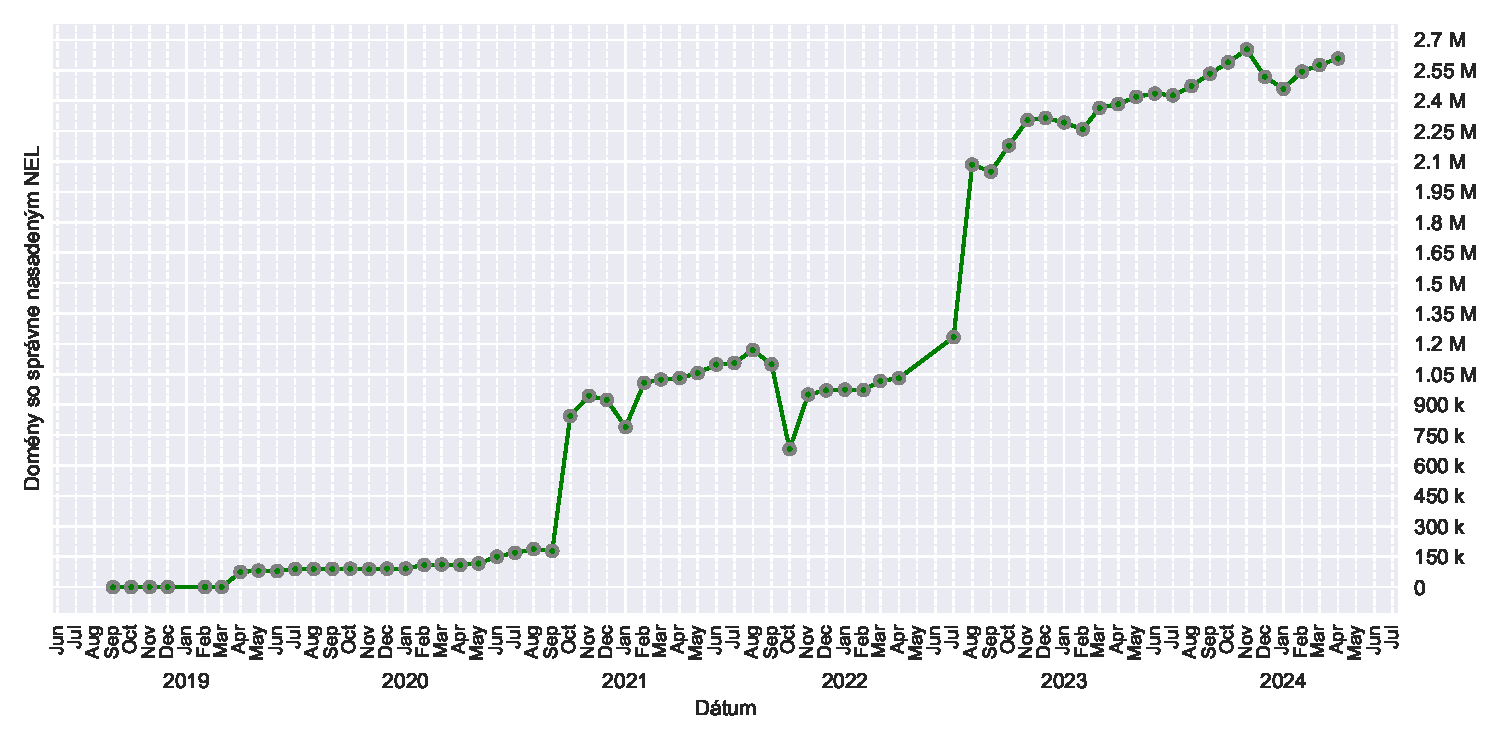
\includegraphics[scale=0.59]{obrazky-figures/httparchive_nel_deployment.pdf}
 \caption{\centering Ale seruuus.}
 \label{fig:httparchive-nel-deployment}
\end{center}
\end{figure}

\pagebreak

\begin{figure}[!htb]
\begin{center}
 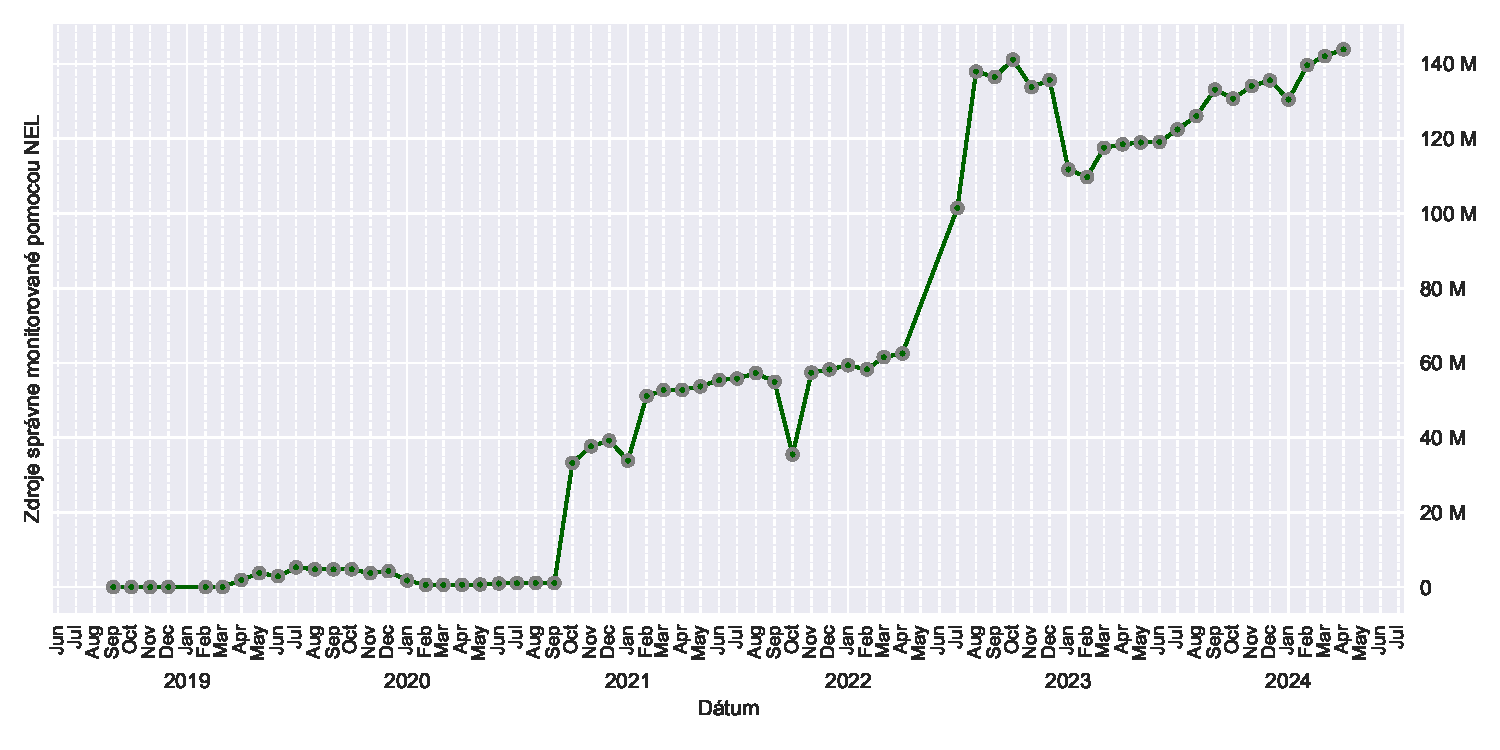
\includegraphics[scale=0.59]{obrazky-figures/httparchive_nel_deployment_resources.pdf}
 \caption{\centering Ale seruuus.}
 \label{fig:httparchive-nel-deployment-resources}
\end{center}
\end{figure}

\pagebreak


\begin{figure}[!htb]
\begin{center}
 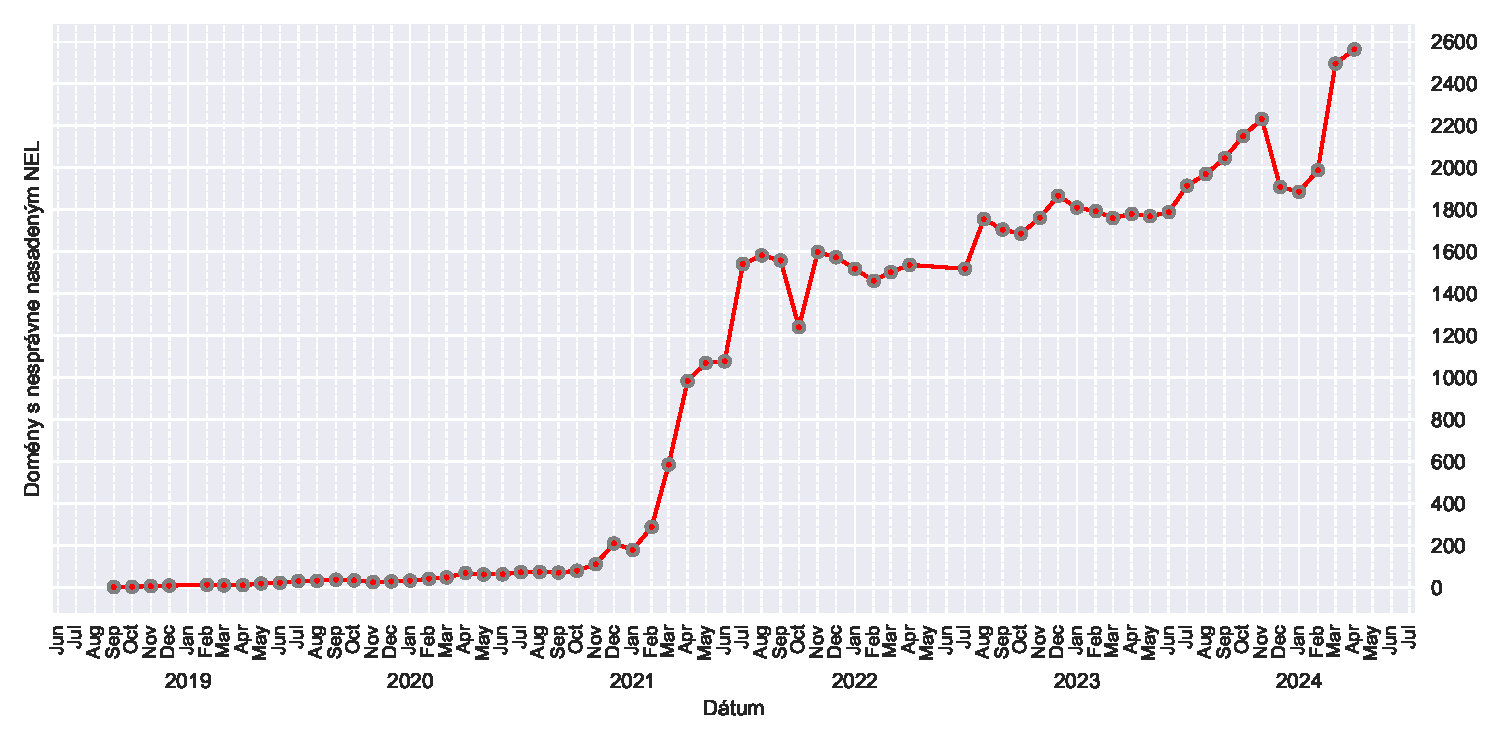
\includegraphics[scale=0.59]{obrazky-figures/httparchive_nel_deployment_incorrect.pdf}
 \caption{\centering Ale seruuus.}
 \label{fig:httparchive-nel-deployment-incorrect}
\end{center}
\end{figure}

\pagebreak


\begin{figure}[!htb]
\begin{center}
 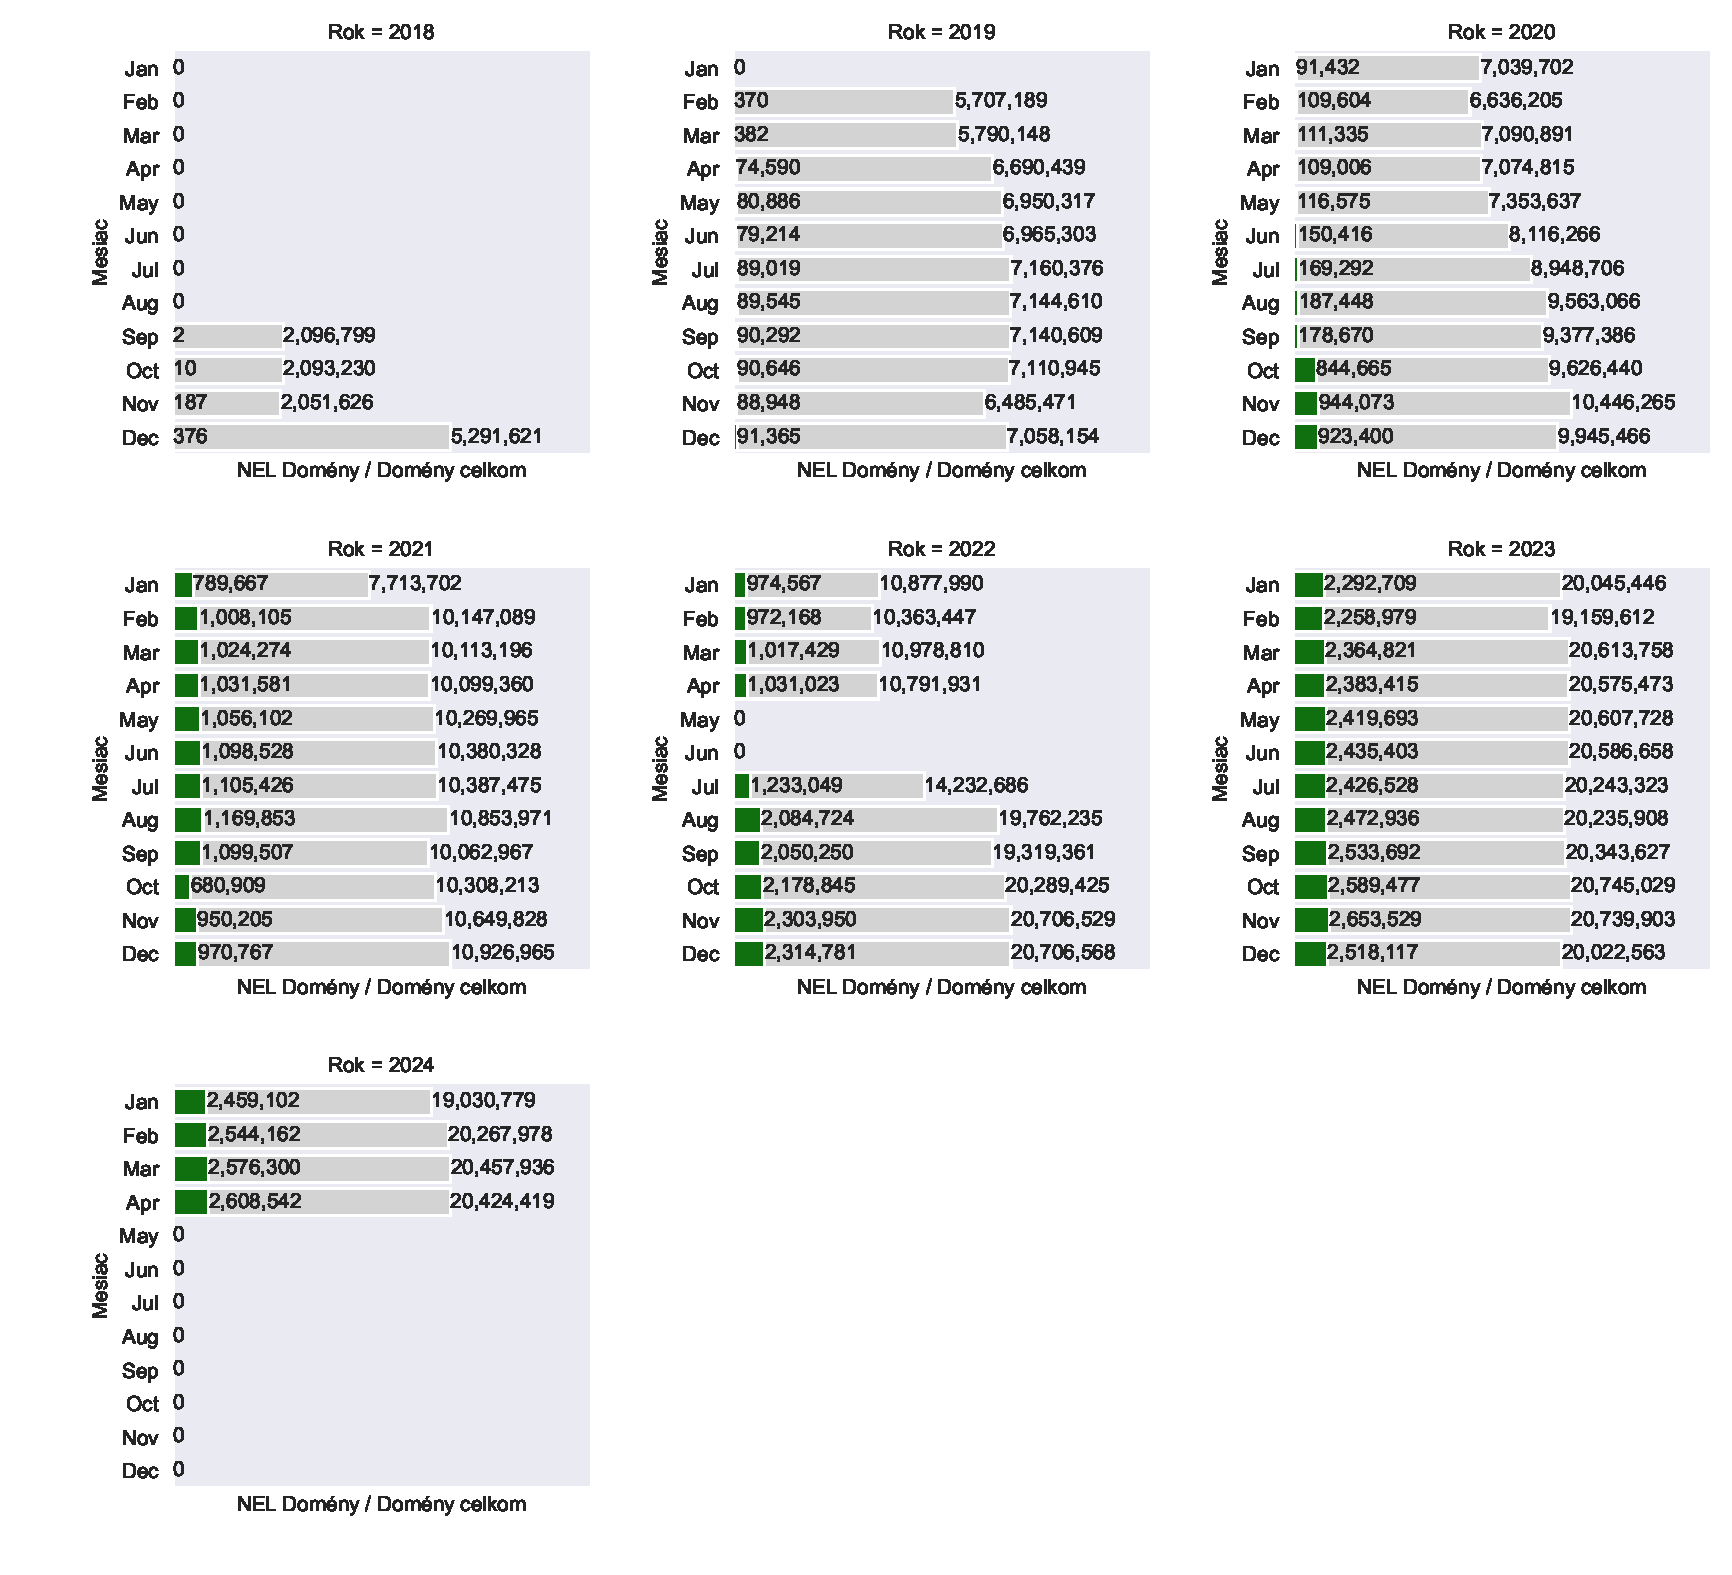
\includegraphics[scale=0.518]{obrazky-figures/httparchive_nel_deployment_ratio_values.pdf}
 \caption{\centering Ale seruuus.}
 \label{fig:httparchive-nel-deployment_ratio_values}
\end{center}
\end{figure}

\pagebreak


\begin{figure}[!htb]
\begin{center}
 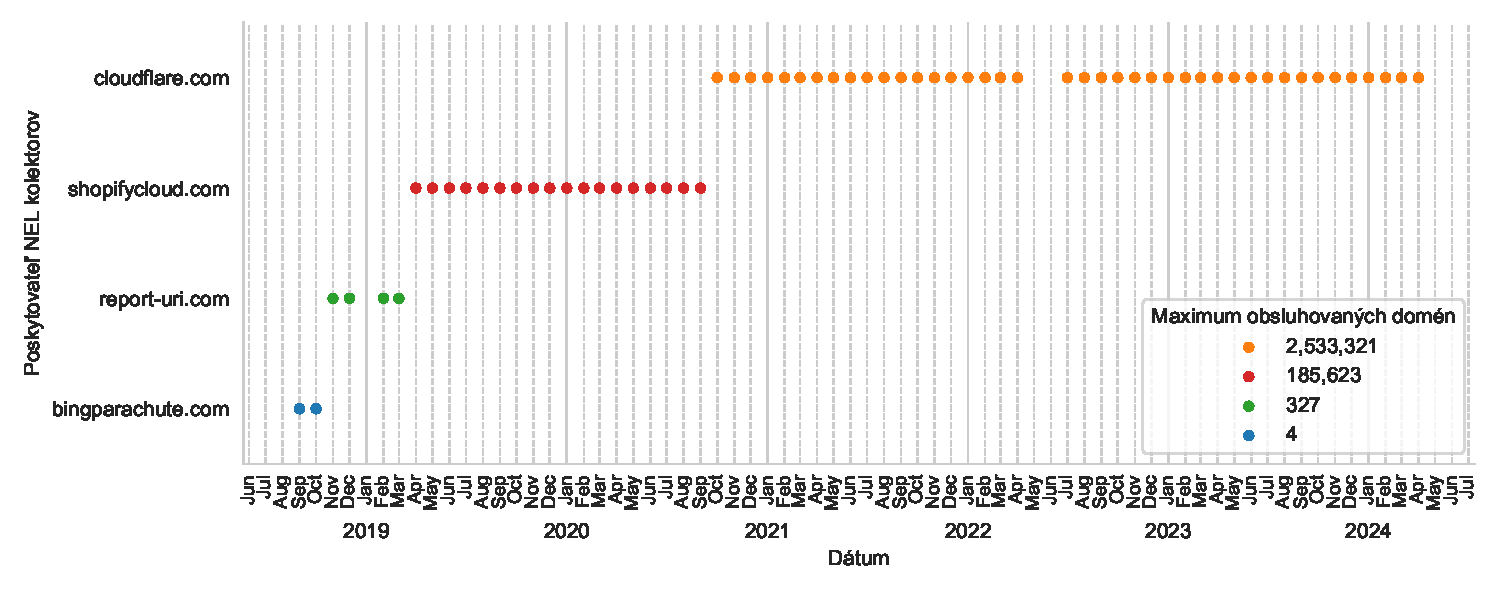
\includegraphics[scale=0.55]{obrazky-figures/httparchive_nel_collector_provider_top_1_over_time.pdf}
 \caption{\centering Ale seruuus.}
 \label{fig:httparchive-nel-collector-provider-top-1-over-time}
\end{center}
\end{figure}

\pagebreak


\begin{figure}[!htb]
\begin{center}
 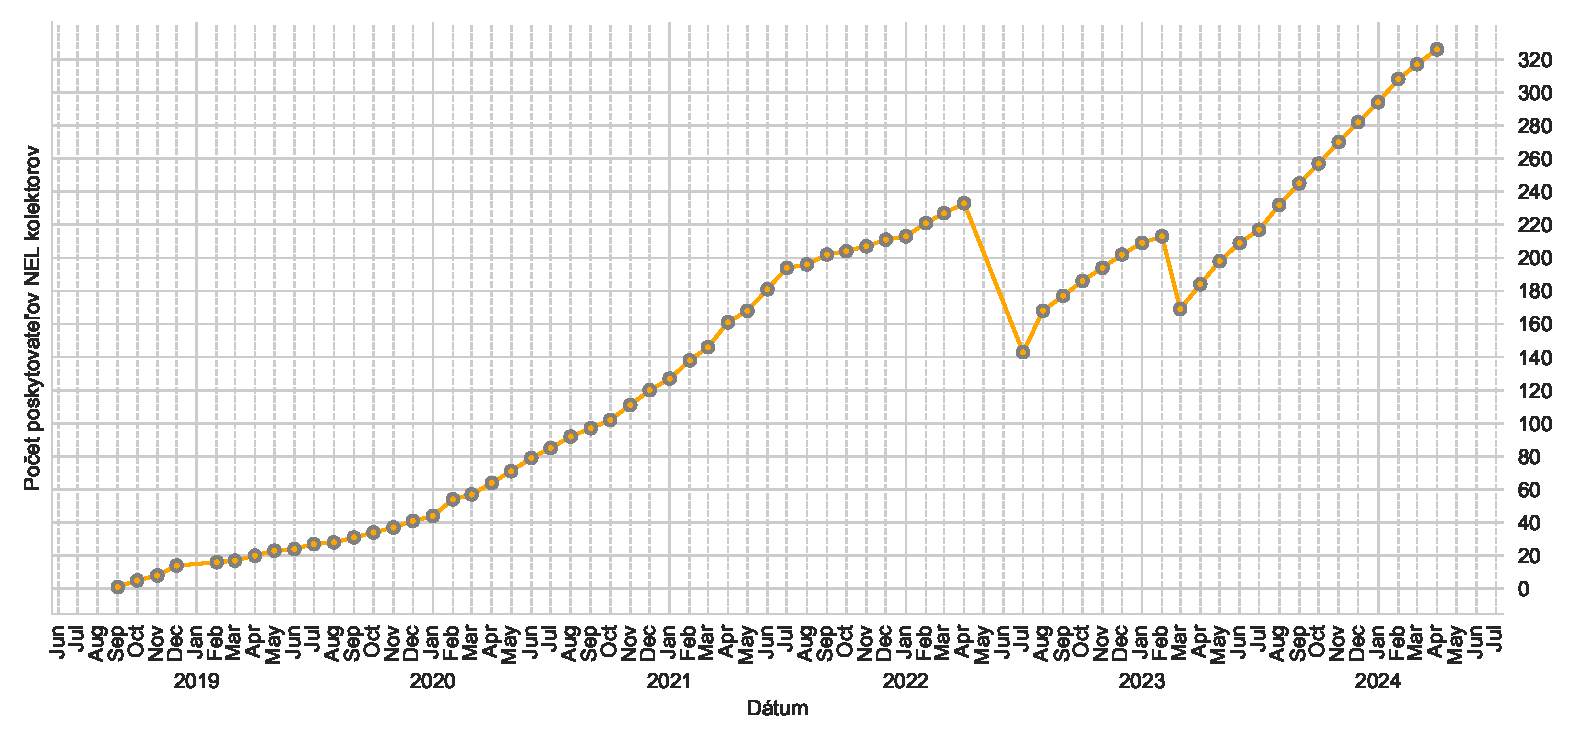
\includegraphics[scale=0.57]{obrazky-figures/httparchive_nel_collector_provider_count.pdf}
 \caption{\centering Ale seruuus.}
 \label{fig:httparchive-nel-collector-provider-top-1-over-time}
\end{center}
\end{figure}

\pagebreak


\begin{figure}[!htb]
\begin{center}
 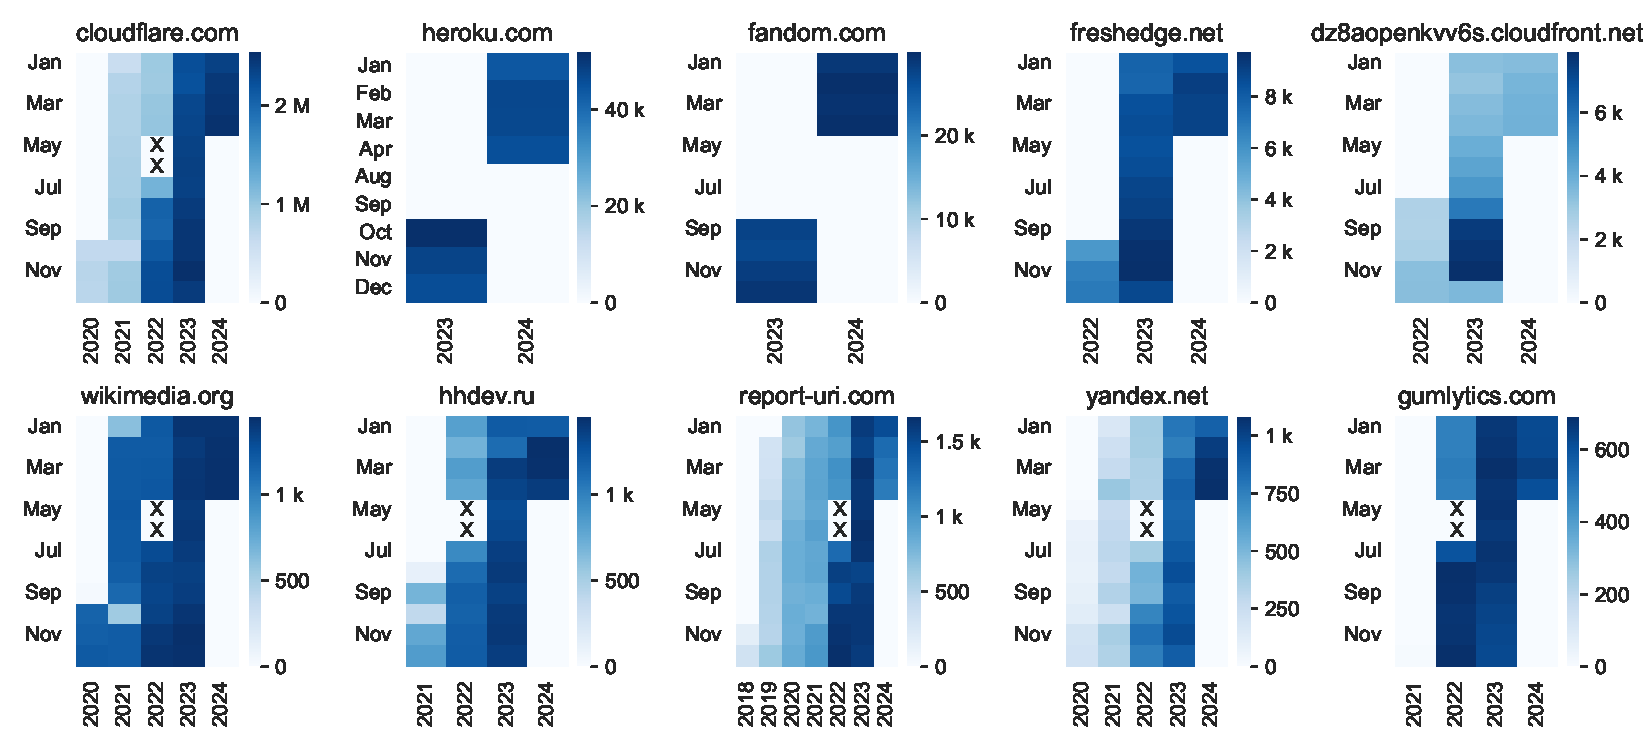
\includegraphics[scale=0.54]{obrazky-figures/httparchive_nel_latest_collector_provider_stats.pdf}
 \caption{\centering Ale seruuus.}
 \label{fig:httparchive-nel-latest-collector-provider-stats}
\end{center}
\end{figure}

\pagebreak


\begin{figure}[!htb]
\begin{center}
 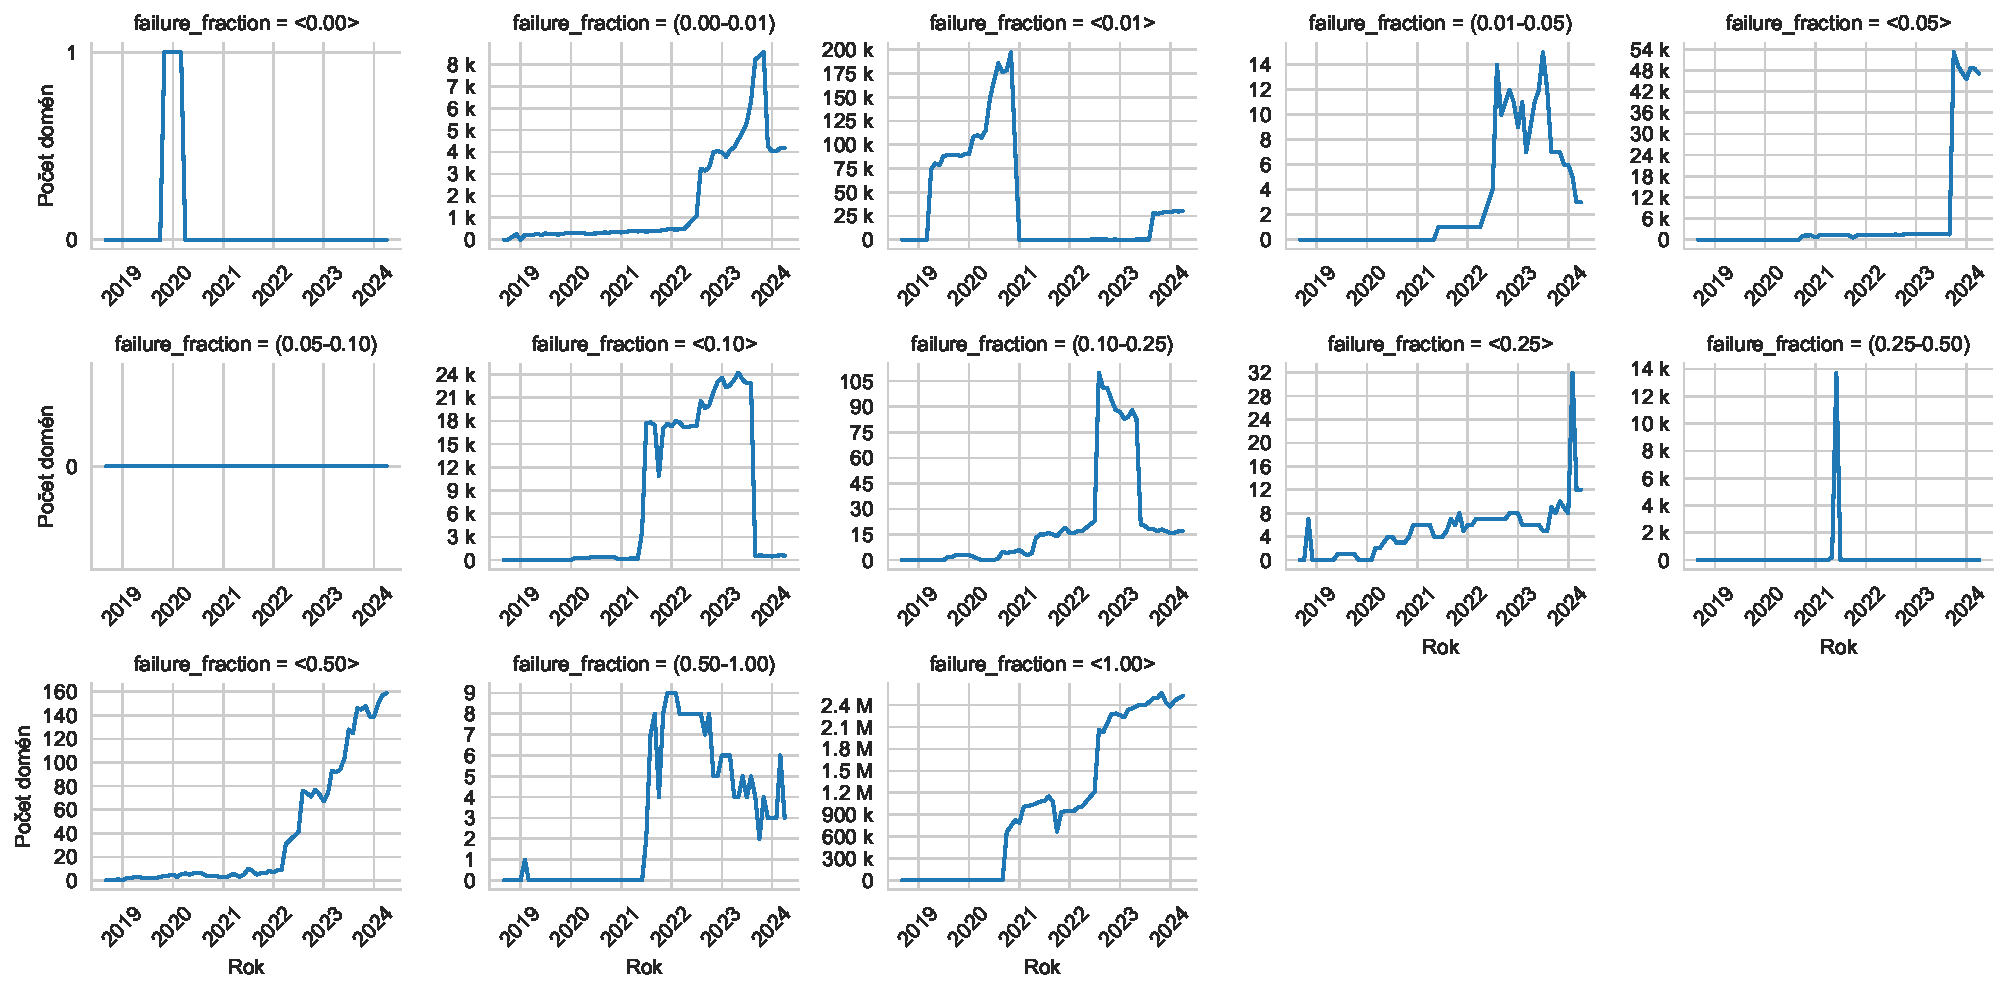
\includegraphics[scale=0.447]{obrazky-figures/httparchive_nel_config_ff_dist.pdf}
 \caption{\centering Ale seruuus.}
 \label{fig:httparchive-nel-config-ff-dist}
\end{center}
\end{figure}

\pagebreak


\begin{figure}[!htb]
\begin{center}
 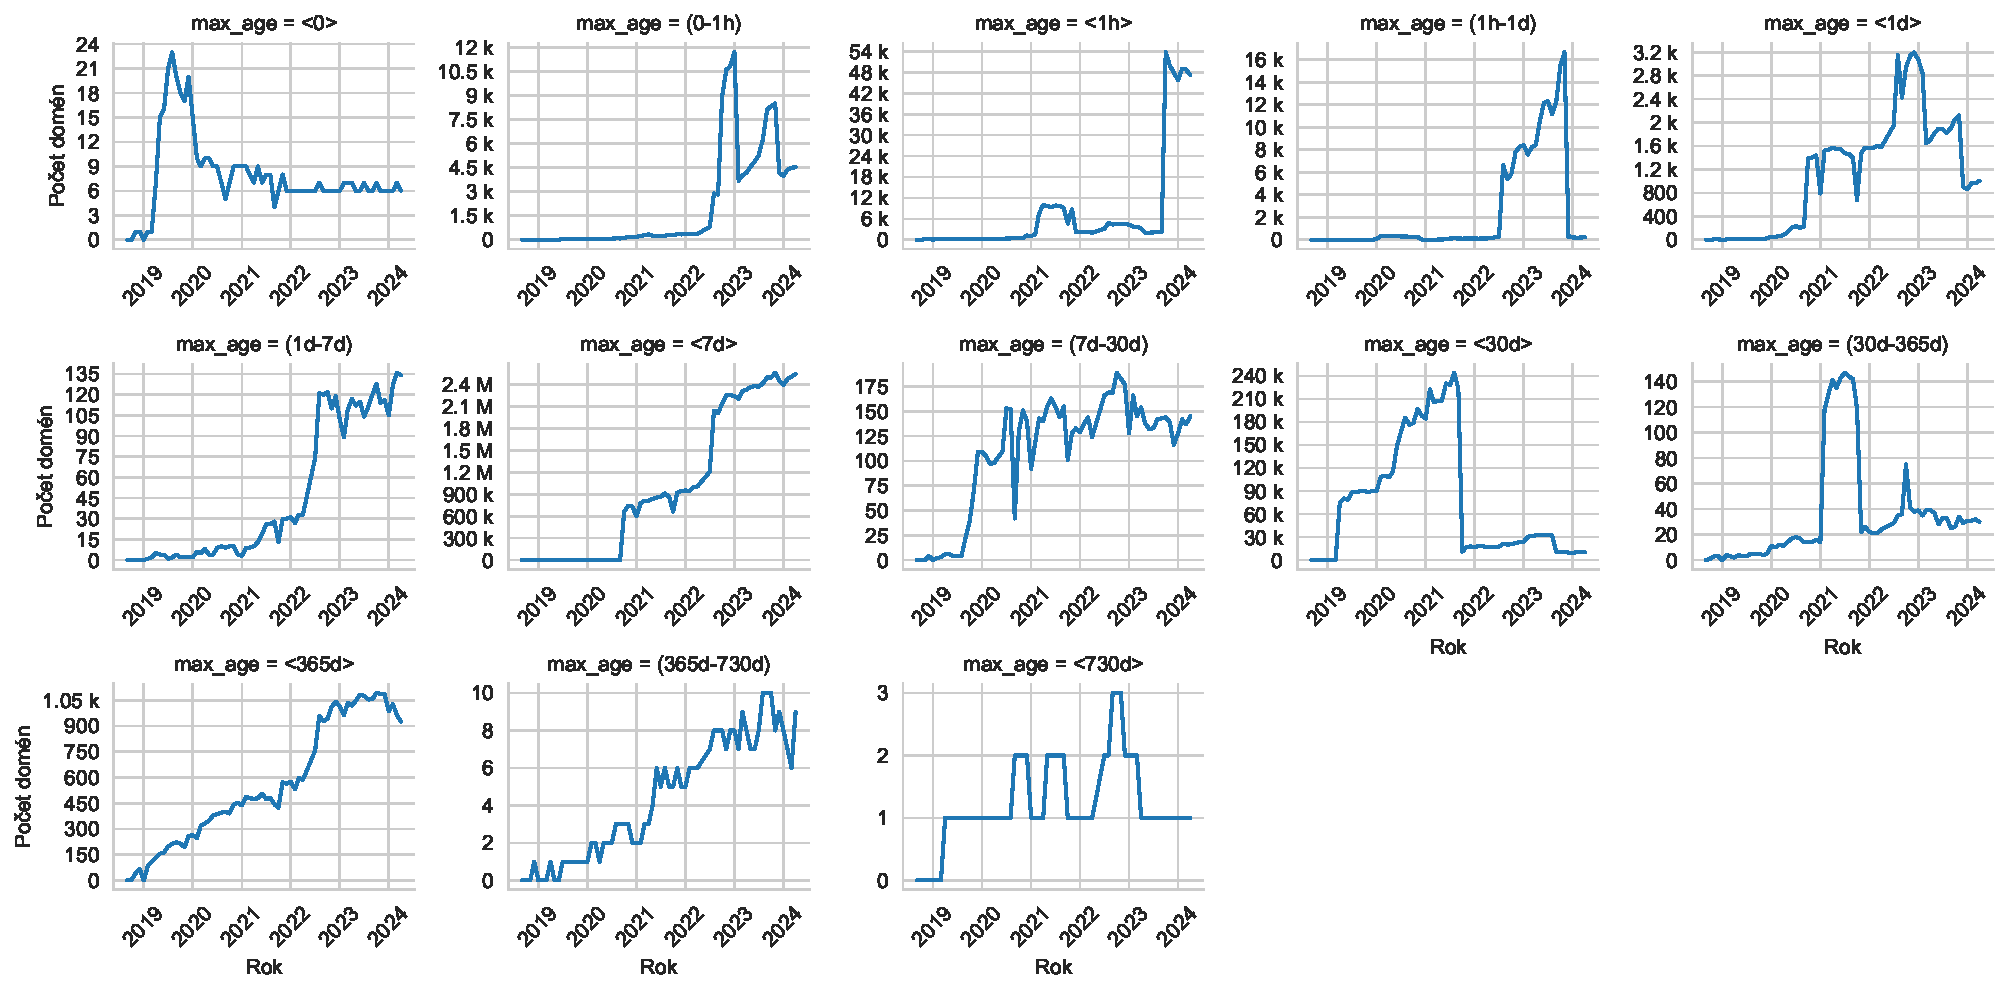
\includegraphics[scale=0.447]{obrazky-figures/httparchive_nel_config_ma_dist.pdf}
 \caption{\centering Ale seruuus.}
 \label{fig:httparchive-nel-config-ma-dist}
\end{center}
\end{figure}

\pagebreak


\begin{figure}[!htb]
\begin{center}
 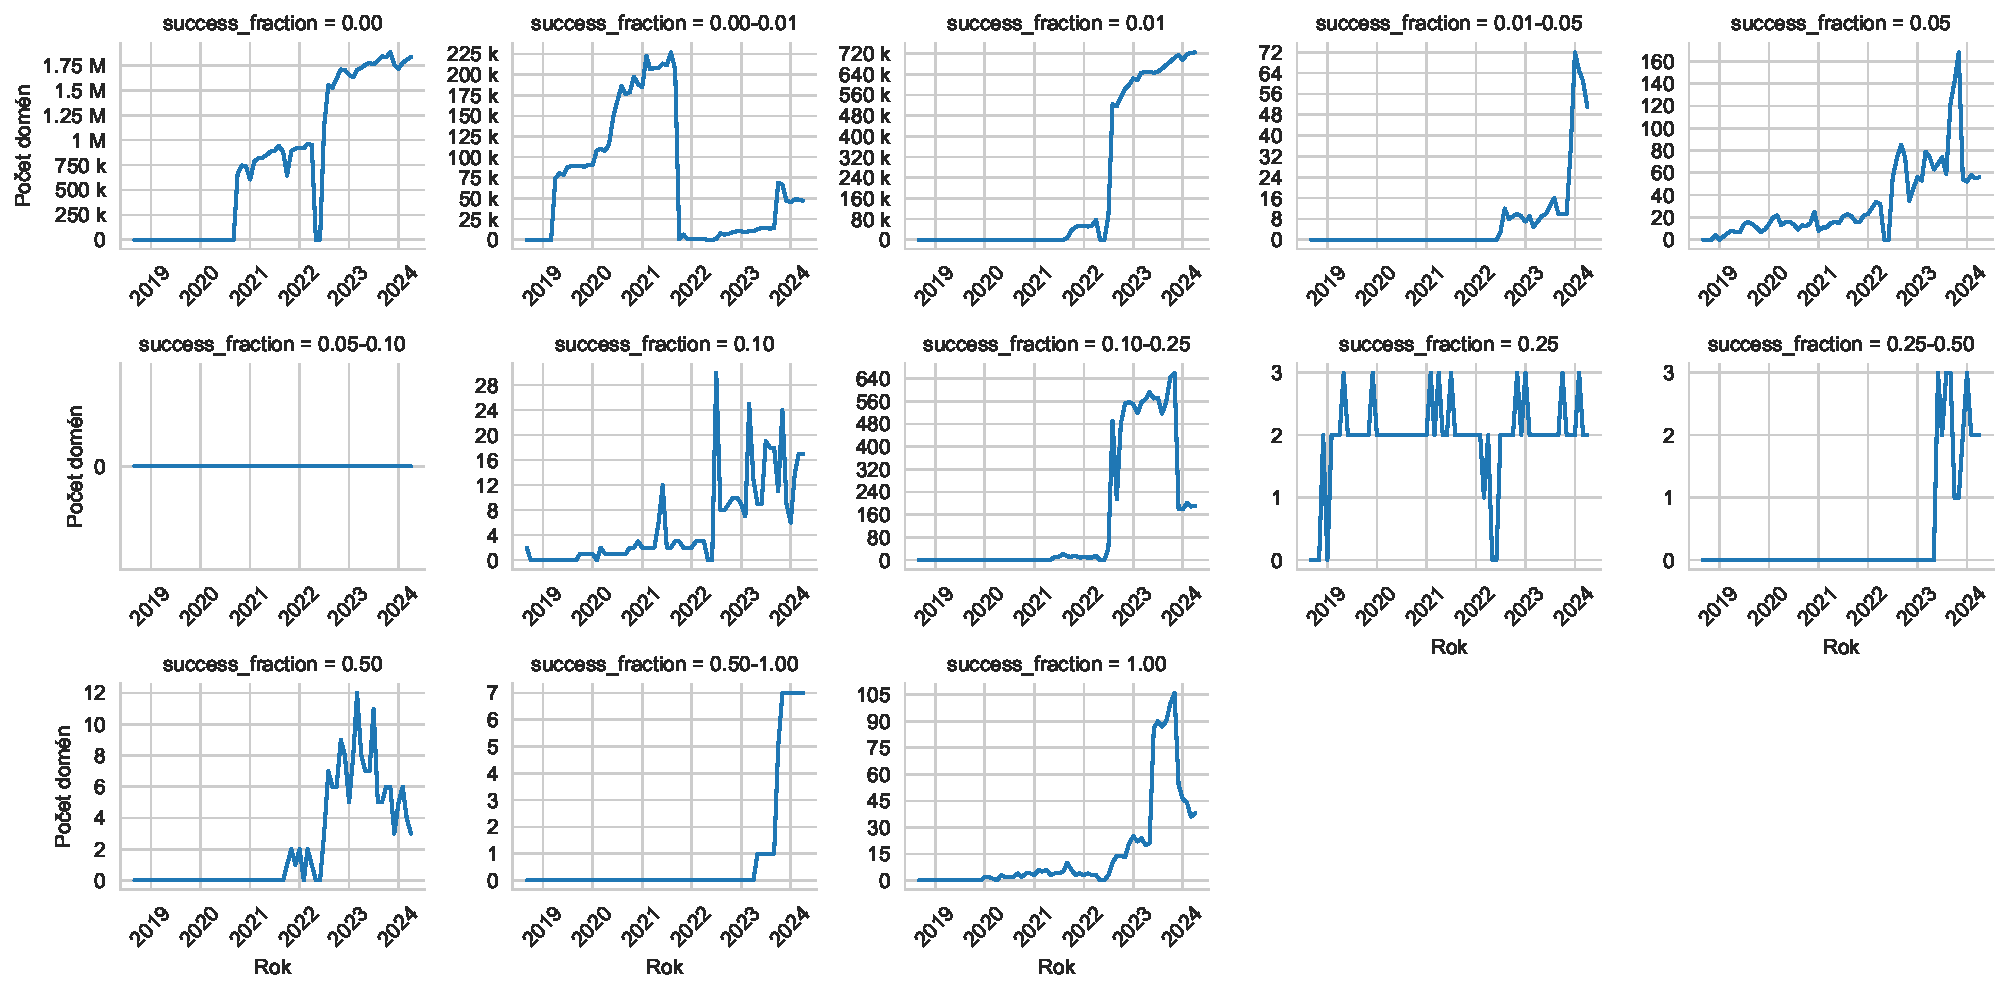
\includegraphics[scale=0.447]{obrazky-figures/httparchive_nel_config_sf_dist.pdf}
 \caption{\centering Ale seruuus.}
 \label{fig:httparchive-nel-config-sf-dist}
\end{center}
\end{figure}

\pagebreak


\begin{figure}[!htb]
\begin{center}
 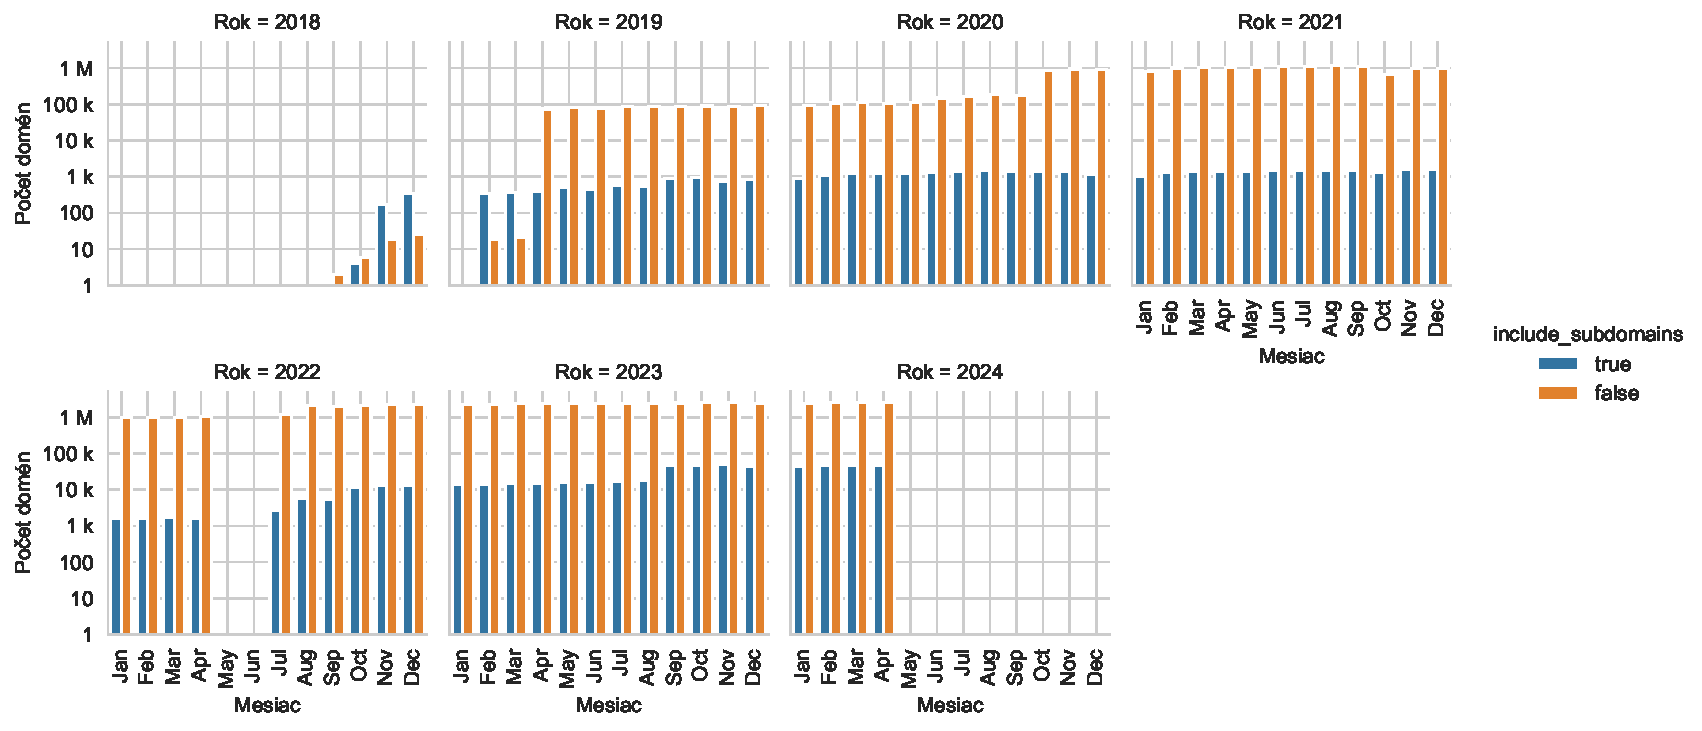
\includegraphics[scale=0.525]{obrazky-figures/httparchive_nel_config_is_dist.pdf}
 \caption{\centering Ale seruuus.}
 \label{fig:httparchive-nel-config-is-dist}
\end{center}
\end{figure}

\pagebreak


\begin{figure}[!htb]
\begin{center}
 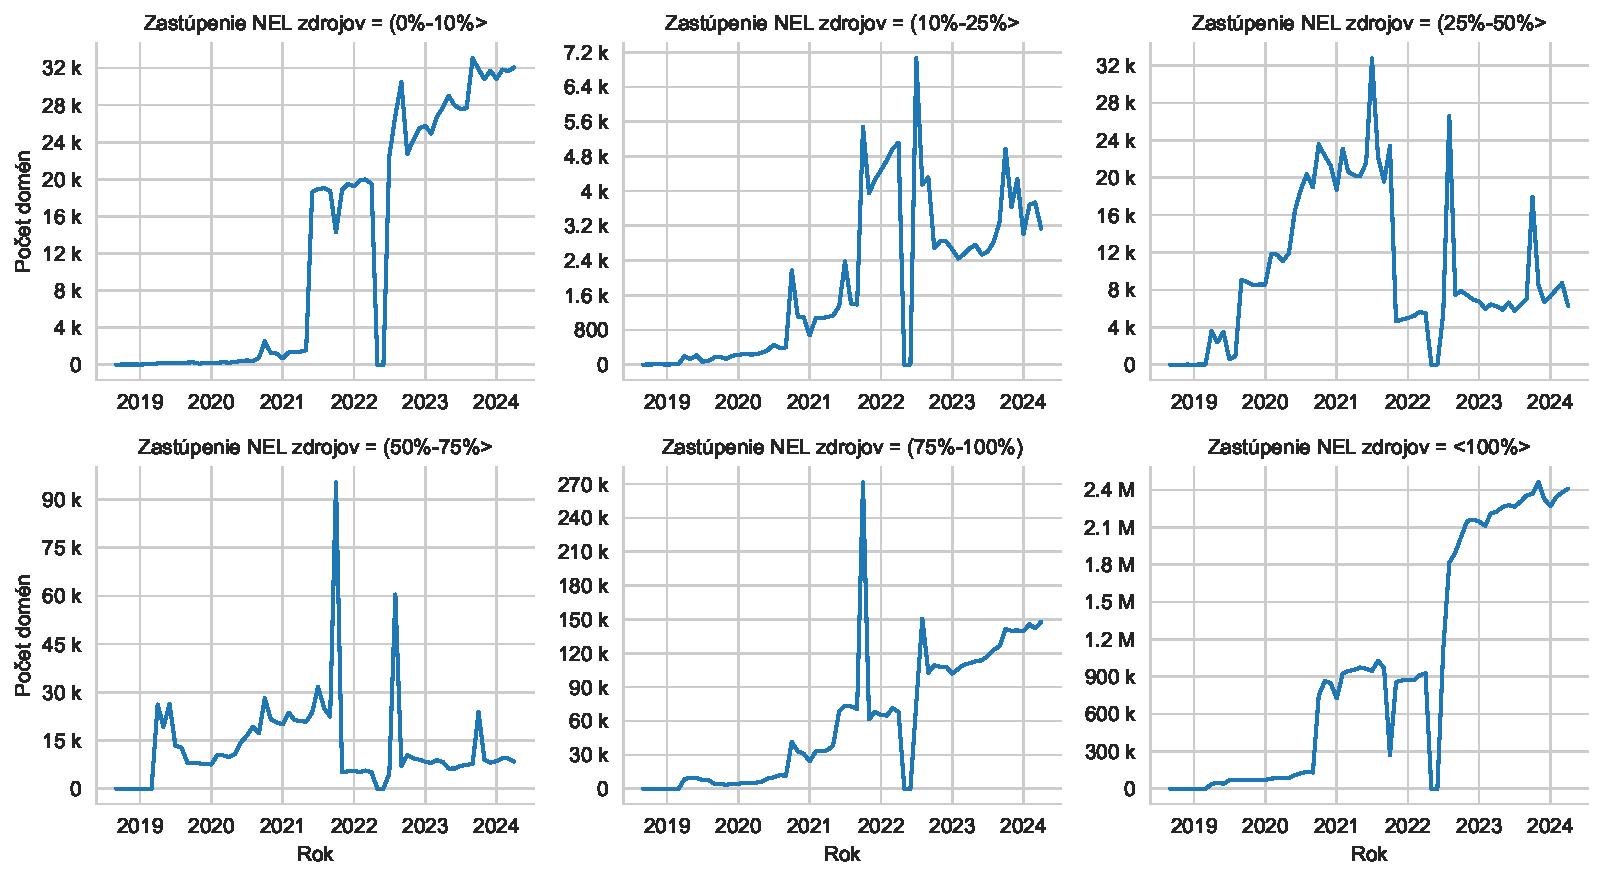
\includegraphics[scale=0.56]{obrazky-figures/httparchive_nel_monitored_resources_percentage_dist.pdf}
 \caption{\centering Ale seruuus.}
 \label{fig:httparchive-nel-monitored-resources-precentage-dist}
\end{center}
\end{figure}

\pagebreak


\begin{table}[!htb]
\centering
\resizebox{\textwidth}{!}{\begin{tabular}{l||r|r|r|r|r|r|r}
\toprule
Dátum & Dec 2018 & Dec 2019 & Dec 2020 & Dec 2021 & Dec 2022 & Dec 2023 & Apr 2024 \\
Počet variácií &  &  &  &  &  &  &  \\
\midrule
\midrule
1 & 375 & 91,355 & 899,292 & 970,362 & 2,293,385 & 2,484,009 & 2,574,899 \\
2 & 2 & 16 & 47,796 & 784 & 42,664 & 67,124 & 66,372 \\
3 & 0 & 6 & 615 & 15 & 51 & 1,563 & 1,317 \\
4 & 0 & 0 & 4 & 0 & 12 & 8 & 4 \\
5 & 0 & 0 & 5 & 0 & 80 & 10 & 5 \\
6 & 0 & 0 & 6 & 0 & 6 & 6 & 6 \\
7 & 0 & 0 & 0 & 0 & 14 & 0 & 0 \\
\bottomrule
\end{tabular}}
\caption{Ale serusendo!}
\end{table}

\pagebreak

\begin{table}[!htb]
\centering
% \resizebox{\textwidth}{!}{
\begin{tabular}{l||r|r|r|r|r}
\toprule
Dátum & IS & FF & SF & MA & Počet domén \\
\midrule
\midrule
Dec 2018 & true & 0.00001 & 0.0 & 3600 & 249 \\
Dec 2019 & false & 0.01 & 0.0001 & 2592000 & 90,373 \\
Dec 2020 & false & 1.0 & 0.0 & 604800 & 732,284 \\
Dec 2021 & false & 1.0 & 0.0 & 604800 & 894,283 \\
Dec 2022 & false & 1.0 & 0.0 & 604800 & 1,680,300 \\
Dec 2023 & false & 1.0 & 0.0 & 604800 & 1,732,435 \\
Apr 2024 & false & 1.0 & 0.0 & 604800 & 1,811,335 \\
\bottomrule
\end{tabular}
% }
\caption{Ale serusendo!}
\end{table}

\pagebreak

\begin{table}[!htb]
\centering
\resizebox{\textwidth}{!}{\begin{tabular}{ll||r|r|r|rr}
\toprule
Dátum & Poskytovateľ & D. nasadenia & Obsluha (nasadenie) & Obsluha (aktuálne) & \% z celku za mesiac \\
\midrule
\midrule
\multirow{10}{*}{Apr 2024} & cloudflare.com & Aug 2020 & 1 & 2,511,907 & 96.273 \\
& heroku.com & Aug 2023 & 2 & 45,405 & 1.740 \\
& fandom.com & May 2023 & 11 & 29,833 & 1.143 \\
& freshedge.net & Oct 2022 & 5,772 & 8,999 & 0.345 \\
& dz8aopenkvv6s.cloudfront.net & Aug 2022 & 2,552 & 3,829 & 0.147 \\
& wikimedia.org & Sep 2020 & 27 & 1,447 & 0.055 \\
& hhdev.ru & Aug 2021 & 120 & 1,385 & 0.053 \\
& report-uri.com & Oct 2018 & 3 & 1,190 & 0.046 \\
& yandex.net & May 2020 & 19 & 1,082 & 0.041 \\
& gumlytics.com & Dec 2021 & 7 & 610 & 0.023 \\
\bottomrule
\end{tabular}}
\caption{Ale serusendo!}
\end{table}